
%(BEGIN_QUESTION)
% Copyright 2014, Tony R. Kuphaldt, released under the Creative Commons Attribution License (v 1.0)
% This means you may do almost anything with this work of mine, so long as you give me proper credit

Se for deg at du bruker et mulitimeter til å måle spenningen mellom ulike punkter i kretsen nedenfor. Om du gjør målingene som bildne viser hva vil mulitimeteret vise?

$$\includegraphics[width=15.5cm]{i01158x01.eps}$$


\begin{itemize}
\item{} $U_{BA} = $
\item{} $U_{DB} = $
\item{} $U_{FD} = $
\item{} $U_{AF} = $
\end{itemize}


\underbar{file i01158}
%(END_QUESTION)





%(BEGIN_ANSWER)

\begin{itemize}
\item{} $U_{BA} = +10.8$ volts
\item{} $U_{DB} = +25.2$ volts
\item{} $U_{FD} = -12.0$ volts
\item{} $U_{AF} = -24.0$ volts
\end{itemize}

%(END_ANSWER)





%(BEGIN_NOTES)

Ask your students this question: ``Will the algebraic sum of voltage measurements ever be other than zero in a loop?''  Ask them to explain {\it why} this is, as best they can.

%INDEX% Electronics review: series-parallel circuits

%(END_NOTES)


